\documentclass[UTF8]{ctexbeamer}
\usetheme{Madrid}
% \usecolortheme{beaver}
\usepackage{hyperref}
\usepackage{graphicx}
\usepackage{wrapfig}
\usepackage{caption}
\usepackage{subcaption}
\DeclareGraphicsExtensions{.eps,.ps,.jpg,.bmp,.png}


\title{初识 Linux}

\author{中国科学技术大学 LUG}

\date{March 15, 2020}

\AtBeginSection[]
{
	\begin{frame}
		\frametitle{Table of Contents}
		\tableofcontents[currentsection]
	\end{frame}
}



\begin{document}

\frame{\titlepage}
\begin{frame}
    % Table of contents 目录/大纲页
    % 自动实现对section的收集,并绘制成目录页
	\frametitle{Table of Contents}
	\tableofcontents
\end{frame}

\section{计算机与操作系统}
\begin{frame}{计算机与操作系统 - 计算机的更新换代}
    \begin{itemize}
        \item 真空管时代(ENIAC) \pause
        \item 晶体管时代(TRADIC) \pause
        \item 集成电路时代(IBM System / 360 系列) \pause
        \item 大规模集成电路时代(Intel 4004) \pause
    \end{itemize}
    现在我们正处于大规模集成电路时代。
\end{frame}

\begin{frame}{计算机与操作系统 - 计算机的更新换代}
    过去几十年,计算机的集成度大幅提升,性能增长呈指数级。
    
    \vspace{1em}
    
    摩尔定律:
    \vspace{0.5em}
    \begin{quote}
    集成电路上可容纳的晶体管数目每两年就会翻一倍。
    
    或者
    
    计算机的性能每 18 个月提高一倍。
    \end{quote}
\end{frame}
\begin{frame}{计算机与操作系统 - 计算机操作系统}
    % Windows
    % macOS
    \begin{figure}
        \centering
        \begin{subfigure}[b]{.4\textwidth}
            \centering
            
\includegraphics[width=\textwidth]{windows}
            \caption{Windows}
            \label{fig:windows}
        \end{subfigure}
        \hfill
        \begin{subfigure}[b]{.4\textwidth}
            \centering
            
\includegraphics[width=\textwidth]{macOS.png}
            \caption{macOS}
            \label{fig:macOS}
        \end{subfigure}
    \end{figure}
    
    \centering
    两大主流的个人计算机操作系统
\end{frame}
\begin{frame}{计算机与操作系统 - 计算机的更新换代}
    
    \begin{itemize}
        \item 计算机最初没有操作系统。
        \begin{itemize}
            \item 最初的计算机不是通用计算机,而是为特定目的服务的专用计算机,因此其架构只需要为这个目的而设计即可,无需操作系统。
            \item 在晶体管时代之前,计算机体积庞大、性能有限,没有能力承载通用的操作系统。
        \end{itemize}
        \item 强大的操作系统在日后诞生并演化。
        \begin{itemize}
            \item 计算机更新换代后,人对计算机的依赖越来越深,需要充分高效地利用计算机自动化的特性。
            \item 计算机的性能足以支撑起一个通用的操作系统。
        \end{itemize}
    \end{itemize}
\end{frame}
\begin{frame}{计算机与操作系统 - 计算机的更新换代}
    计算机操作系统的功能:
    
    \begin{itemize}
        \item 进程管理
        \item 内存管理
        \item 文件系统
        \item 网络通信
        \item 安全机制
        \item 用户界面
        \item 驱动程序
    \end{itemize}
    \vspace{1em}
    操作系统成为了联络用户和底层硬件的中介,让用户无需关心底层硬件即可使用计算机,大幅降低了使用的学习成本。

    操作系统也是如今我们和计算机打交道必不可少的工具。
\end{frame}
\section{什么是 Linux?}
\begin{frame}{什么是 Linux - Linux 的起源}

    \begin{columns}
    \column{0.6\textwidth}
    \begin{itemize}
        \item 1969 年,贝尔实验室开发了 UNIX 操作系统,得到了学院和企业的广泛使用。
        \item 期间许多从业人士都基于它开发了衍生的组件和变种系统。
        \item UNIX 最初虽然开源,但随后改变了策略,收回了授权并对所有了衍生作品进行了著作权诉讼。
        \item 许多过去的用户都对此十分不满,并期待一个更自由的系统出现。
    \end{itemize}
    \column{0.4\textwidth}
    \begin{figure}
        
\includegraphics[width=\textwidth]{unix.png}
        \caption{Unix}
        \label{fig:unix}
    \end{figure}
    
    \end{columns}

\end{frame}
\begin{frame}{什么是 Linux - Linux 的起源}
    \begin{columns}
    \column{0.6\textwidth}
    \begin{itemize}
        \item 1983 年,麻省理工学院的理查德·斯托曼对了对抗 UNIX 的行径,发动了 GNU 计划,希望创建一个类似 UNIX 但完全自由的操作系统。
        \item 这个计划没能完全实现,但孕育出了很多日后经典的开源工具(比如说 Emacs)。
        \item 这个计划中诞生了有名的 GNU 通用公共许可证(GPL),保证 GNU 软件可以自由地时使用、修改和分发。这形成了一个新的版权概念:著作传。
    \end{itemize}
    \column{0.4\textwidth}
    \begin{figure}
        \centering
        
\includegraphics[width=\textwidth]{GNU.png}
        \caption{GNU = GNU's not UNIX}
        \label{fig:gnu}
    \end{figure}
    \end{columns}
\end{frame}
\begin{frame}{什么是 Linux - Linux 的起源}
    \begin{columns}
    \column{0.4\textwidth}
    \begin{figure}
        \centering
        
\includegraphics[width=\textwidth]{Tux.png}
        \caption{Tux}
        \label{fig:linux}
    \end{figure}
    \column{0.6\textwidth}
    \begin{itemize}

        \item 1991 年,正在读大学的林纳斯·托瓦兹对 MINIX 系统不能用于商业十分不满,于是自己写了一个操作系统。
        \item 这个操作系统就是 Linux 内核,是日后众多 Linux 发行版的核心模块。
        \item Linux 内核不是一个现代意义的操作系统,但通过各方人士的贡献,诞生出了许多基于它的操作系统,这些系统就被称为“Linux 发行版”。
    \end{itemize}

    \end{columns}
    
\end{frame}
\begin{frame}{什么是 Linux - Linux 发行版}
    \begin{itemize}
        \item 一个典型的 Linux 发行版除了 Linux 内核以外,通常还会包括:
        \begin{itemize}
            \item 一系列工具(比如 GNU 组件)和库
            \item 一些自带的软件
            \item 说明文档
            \item 桌面系统
            \item 窗口管理器
            \item 桌面环境
        \end{itemize}
    \end{itemize}
    
    % Debian 分支
    % RedHat 分支
    % Arch Linux 分支
\end{frame}

\begin{frame}{Debian 分支}
    \begin{figure}
        \centering
        
\includegraphics[width=0.4\textwidth]{debian.png}
        \caption{Debian}
        \label{fig:debian}
    \end{figure}
    Debian 是一个完全由自由软件构成的类 UNIX 操作系统,第一个版本发布于 1993 年 9 月 15 日,迄今仍在维护,是最早的发行版之一。其以坚持自由软件精神和生态环境优良而出名,拥有庞大的用户群体,甚至自己也成为了一个主流的子框架,称为“Debian GNU/Linux”。
\end{frame}
\begin{frame}{Debian 分支}
    \begin{figure}
        \centering
        
\includegraphics[width=0.4\textwidth]{ubuntu.png}
        \caption{Ubuntu}
        \label{fig:ubuntu}
    \end{figure}
    Debian GNU/Linux 也派生了很多发行版,其中最为著名的便是 Ubuntu(官方译名“友邦拓”)。Ubuntu 由英国的 Canonical 公司主导创立,是一个主打桌面应用的操作系统。其为一般用户提供了一个时新且稳定的由自由软件构成的操作系统,且拥有庞大的社群力量和资源,十分适合普通用户使用。
\end{frame}
\begin{frame}{Red Hat 分支}
    \begin{figure}
        \centering
        
\includegraphics[width=0.4\textwidth]{redhat.png}
        \caption{Red Hat}
        \label{fig:redhat}
    \end{figure}
    Red Hat Linux 是美国的 Red Hat 公司发行的一个发行版,第一个版本发布于 1994 年 11 月 3 日,也是一个历史悠久的发行版。它曾经也广为使用,但在 2003 年 Red Hat 公司停止了对它的维护,转而将精力都投身于其企业版 Red Hat Enterprise Linux(简称 RHEL)上,Red Hat Linux 自此完结,而商业市场导向的 RHEL 维护至今。
\end{frame}
\begin{frame}{Red Hat 分支}
    \begin{figure}
        \centering
        
\includegraphics[width=0.4\textwidth]{fedora.png}
        \caption{Fedora}
        \label{fig:fedora}
    \end{figure}
    在 Red Hat Linux 在停止官方更新后,由社群启动的 Fedora 项目接管了其源代码并构筑了自己的更新,演变成了如今的 Fedora 发行版。Fedora 是一套功能完备且更新迅速的系统,且本身计划也受到了 Red Hat 公司的赞助,成为了公司测试新技术的平台。
\end{frame}
\begin{frame}{Red Hat 分支}
    \begin{figure}
        \centering
        
\includegraphics[width=0.4\textwidth]{centos.png}
        \caption{CentOS}
        \label{fig:centos}
    \end{figure}
    虽然 RHEL 是一个收费的、商业化的系统,但是其遵循 GNU 通用公共许可证,因此会开放源代码。编译这些源代码可以重新得到一个可以使用的操作系统,因此通过这种方法,就得到了一个新的发行版:CentOS,其全称是 Community Enterprise Operating System(社区版企业操作系统)。可以认为 CentOS 大体上就是一个 RHEL 的免费的社区复刻。因为 CentOS 几乎完全编译自 RHEL 的代码,所以其也像 RHEL 一样具有企业级别的稳定性,适合在要求高度稳定的服务器上运行。
\end{frame}
\begin{frame}{Arch Linux 分支}
    \begin{figure}
        \centering
        
\includegraphics[width=0.4\textwidth]{archlinux.png}
        \caption{Arch Linux}
        \label{fig:archlinux}
    \end{figure}
    Arch Linux 是一个基于 x86-64 架构的 Linux 发行版,不过因为其内核默认就包含了部分非自由的模块,所以其未受到 GNU 计划的官方支持。即便如此,Arch Linux 也因其“简单、现代、实在、人本、万能”的宗旨赢得了 Linux 中坚用户的广泛青睐。
\end{frame}
\begin{frame}{Arch Linux 分支}
    \begin{figure}
        \centering
        
\includegraphics[width=0.4\textwidth]{archlinux.png}
        \caption{Arch Linux}
    \end{figure}
    不过,Arch Linux 对这个宗旨的定义和其它发行版有所区别。通常的操作系统为了方便用户快速上手,都是尽可能隐藏底层细节,从而避免用户了解操作系统的运行知识即可直接使用。但是 Arch Linux 则是重在构建优雅、极简的代码结构,这方便了使用者去理解系统,但不可避免地要求使用者自身愿意去了解操作系统的运作方式。某种程度上说,它的“简单”和“人本”注重的是方便用户通过了解而去最大化地利用它,而不是采取屏蔽工作原理的方式来降低使用门槛。因此,本书不建议初学者直接上手 Arch Linux,但十分推荐在读者对 Linux 有进一步了解之后去探索它。
\end{frame}
\begin{frame}{Arch Linux 分支}
    \begin{figure}
        \centering
        
\includegraphics[width=0.4\textwidth]{manjaro.png}
        \caption{Manjaro}
        \label{fig:manjaro}
    \end{figure}
    Arch Linux 拥有强大的功能,但因其特殊的理念使得用户不易使用。为了能让一般用户也能用上 Arch Linux 的强大功能,它的变种 Manjaro 发行版于 2011 年问世。Manjaro 发行版基于 Arch Linux,但更注重易用,因而更适合一般用户。
\end{frame}
\begin{frame}{什么是 Linux - 总结}
    与 Windows 或者 MacOS 比较单一和线性的发展轨迹不同,Linux 发展进程必定是一个去中心化的、非线性的形式。

    什么是 Linux?
    \begin{itemize}
        \item 它可以指代 Linux 内核
        \item 也可能指代一个或者多个 Linux 发行版。
    \end{itemize}
\end{frame}
\section{我们身边的 Linux}
\begin{frame}{我们身边的 Linux}
    实际上,Linux 的各类发行版其实早已深入我们的日常生活。
    % 智能手机
    % 服务器
    % 电视机顶盒
\end{frame}

\begin{frame}{智能手机}
    
    \begin{columns}
    \column{0.3\textwidth}
    \begin{figure}
        \centering
        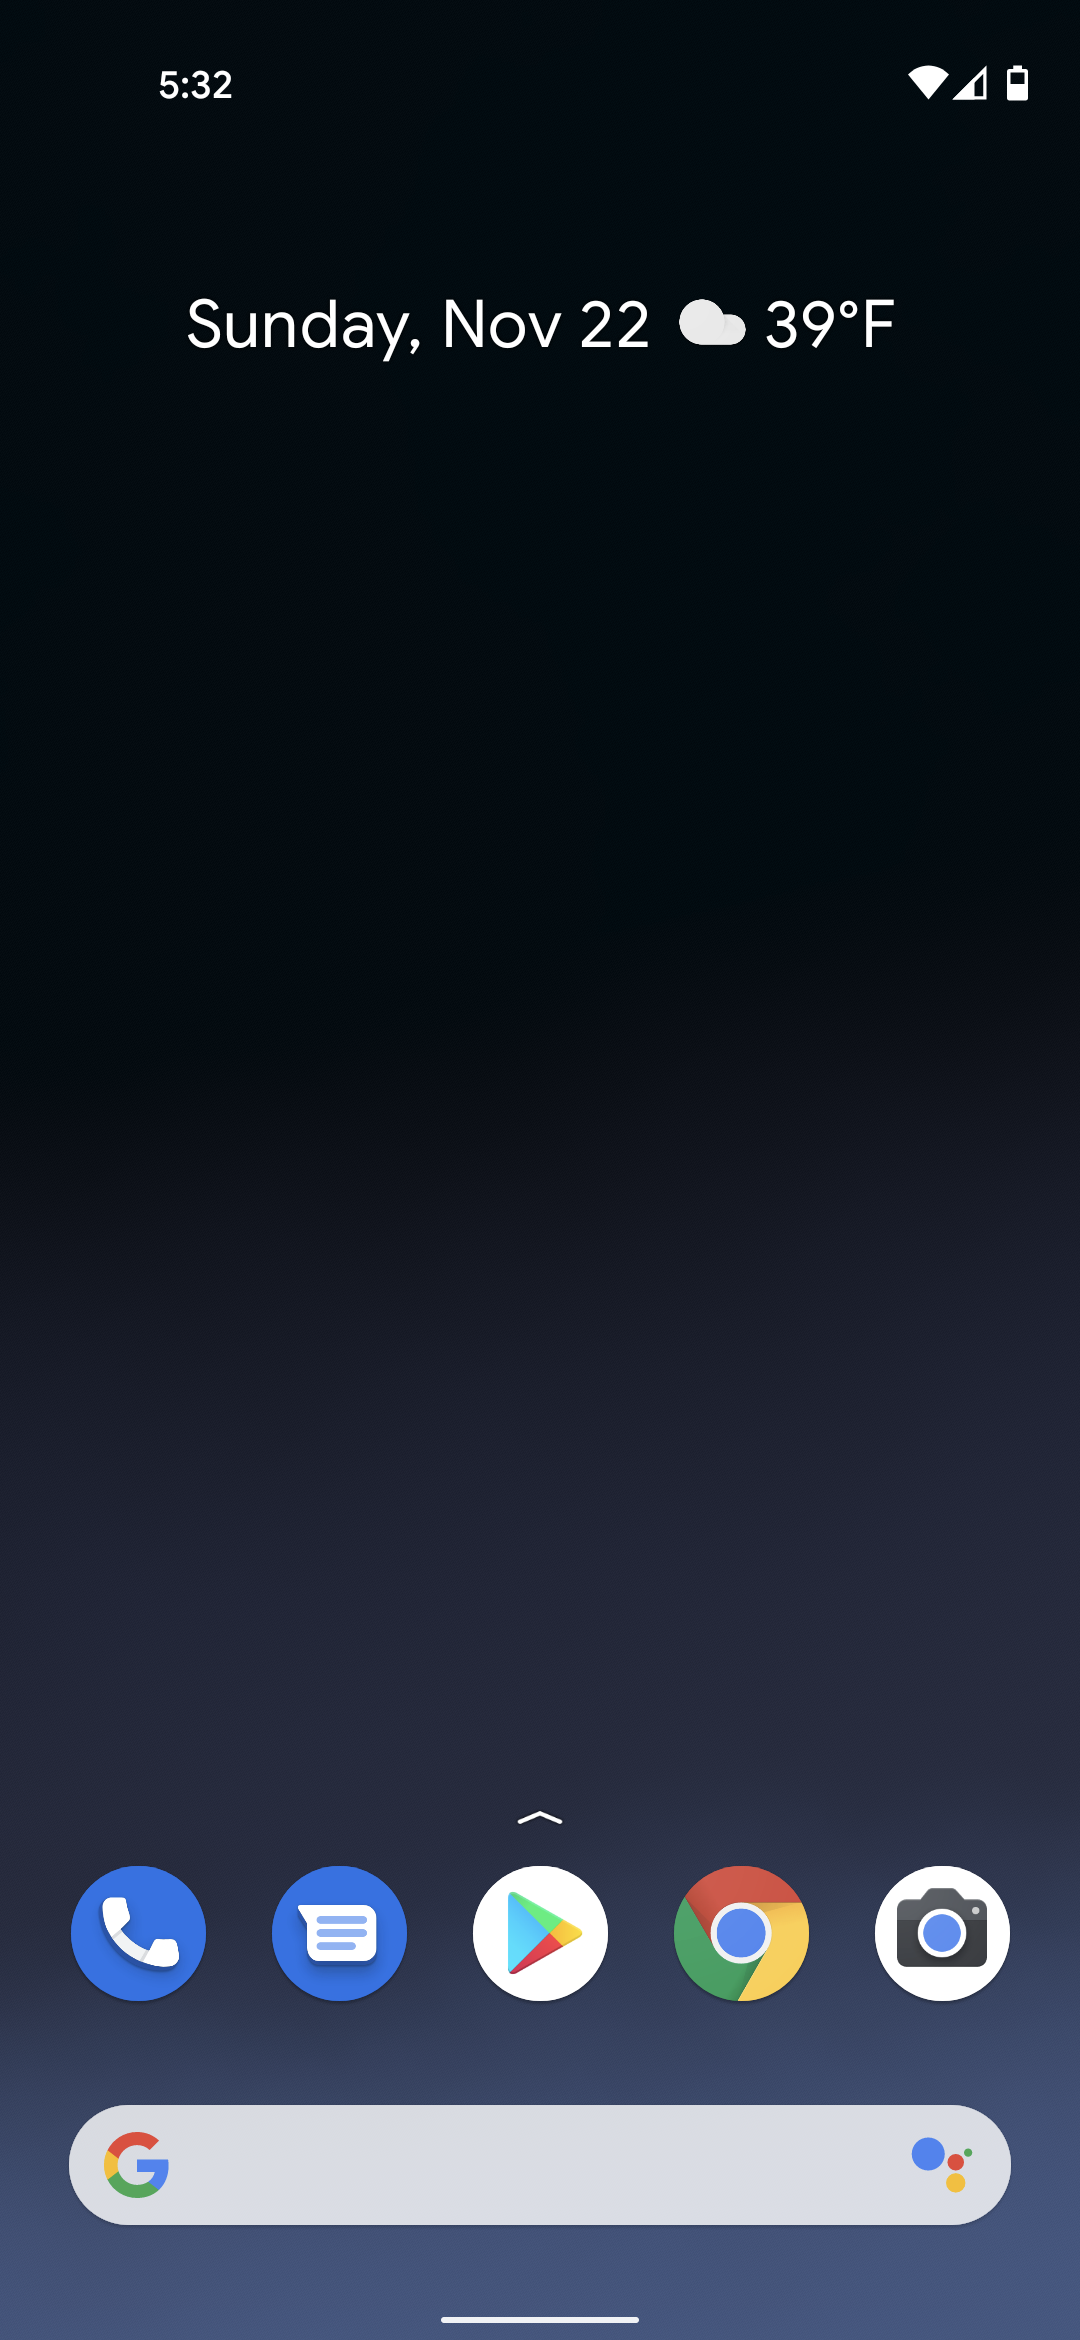
\includegraphics[width=0.8\textwidth]{android.png}
        \caption{Android}
        \label{fig:android}
    \end{figure}
    \column{0.65\textwidth}
    \begin{itemize}
        \item 智能手机目前两个主流的操作系统:
        \begin{itemize}
            \item 苹果公司的 iOS
            \item 谷歌公司的 Android
        \end{itemize}
        \item Android 正是 Linux 的一个知名的发行版,属于 Android / Linux 分支。
        \item 由谷歌公司推出的 叫做 Android 原生系统,基于它诞生出来的操作系统就是 Android / Linux 系下的子发行版,如:
        \begin{itemize}
            \item 华为公司的 EMUI
            \item 小米公司的 MIUI
            \item 锤子科技的 Smartisan OS
        \end{itemize}
    \end{itemize}
    \end{columns}
    
\end{frame}
\begin{frame}{服务器}
    我们的生活离不开互联网。我们可以使用互联网提供的服务搜寻资料、在线办公、亲友社交等等。这些服务都需要远程的计算机提供,这些计算机就是服务器。
    
    服务器更青睐各类 Linux 发行版作为操作系统,比如 RHEL 和 CentOS。
    
    另一类服务器操作系统是微软公司的 Windows Server 系列。
    
    \begin{figure}
        \centering
        
\includegraphics[width=0.4\textwidth]{windows-server-logo.png}
        \caption{Windows Server}
        \label{fig:windows-server}
    \end{figure}
\end{frame}
\begin{frame}{电视机顶盒}
    
    \begin{figure}
        \centering
        
\includegraphics[width=0.6\textwidth]{androidtv.png}
        \caption{Android TV}
        \label{fig:androidtv}
    \end{figure}
    现在很多家庭都会安装带有机顶盒的智能数字电视,实际上顶盒就是一个嵌入式设备。

    Android / Linux 分支下的各类发行版正是主流的嵌入式操作系统,如谷歌公司的 Android TV 操作系统。
\end{frame}
\section{让自己的计算机用上 Linux}
\begin{frame}{让自己的计算机用上 Linux}
    在学习 Linux 的时候,手头准备一个随时可用的 Linux 发行版非常重要。

    强烈建议在本机安装一个属于自己的 Linux 发行版供随时实践。

    在本机上安装一个 Linux 发行版的实现方式有很多,如:
    \begin{itemize}
        \item 安装方法可以选择实机安装或虚拟机安装
        \item 发行版则可以在诸多选项中任意抉择
    \end{itemize}
\end{frame}
\begin{frame}{让自己的计算机用上 Linux}
    推荐采用在虚拟机上运行安装完毕的镜像的方式来安装你的第一个 Linux 系统。这么做的优点有:
    \begin{itemize}
        \item 不需要更改计算机操作系统的引导设置。
        \item 很多情况下避免了硬件兼容性问题。
        \item 安装流程已提前完成,不用经历安装步骤。
        \item 就算在虚拟机中玩脱,也不会引火烧身,且可以随时重置修复。
        \item 在学习 Linux 时依然能快乐地使用现在惯用的操作系统。
    \end{itemize}
\end{frame}
\begin{frame}{让自己的计算机用上 Linux}


    \begin{columns}
    
    \column[t]{0.4\textwidth}
    % vmware
    推荐的虚拟机管理软件
    
    免费,支持中文
    \begin{figure}
        \centering
        
\includegraphics[width=0.8\textwidth]{vmware.png}
        \caption{vmware}
        \label{fig:vmware}
    \end{figure}
    
    \begin{figure}
        \centering
        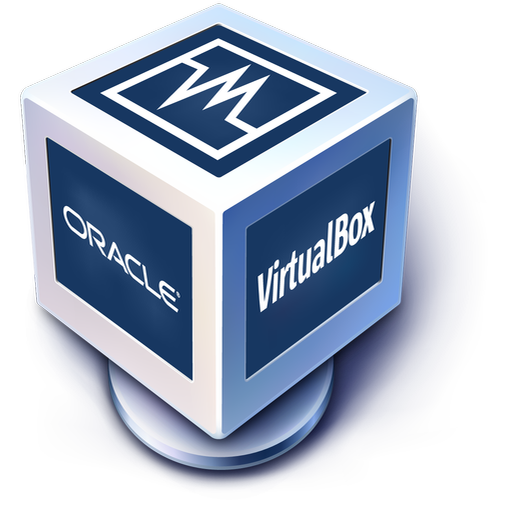
\includegraphics[width=0.3\textwidth]{virtualbox.png}
        \caption{Virtual Box}
        \label{fig:virtualbox}
    \end{figure}
    
    \column[t]{0.4\textwidth}
    % xubuntu
    
    推荐的发行版:Xubuntu
    
    Ubuntu 的子发行版
    
    更轻量、兼容性更高
    
    \begin{figure}
        \centering
        
\includegraphics[width=\textwidth]{xubuntu.png}
        \caption{Xubuntu}
        \label{fig:xubuntu}
    \end{figure}
    \end{columns}

\end{frame}
\end{document}
